\section{Knowledge is Fragile}

Knowledge that is generated via empiricism, bottom-up induction method, is ``the best we've got'', since it's grounded on reality and practicality, as opposed to top-down plain theory generation via deductive reasoning.

Empirical based knowledge generation can be self-correcting, meaning that we know that we're going to be fooled in the learning process and that errors will be made, but we will eventually figure it out along the way and fine tune our knowledge base, thus getting closer and closer to ``the truth''.

Having said that, there are several shortcomings that must be understood about the fragility of knowledge, specially when applied to complex systems (with non-linear responses).

\subsection{Absence of evidence vs evidence of absense}
No amount of empirical evidence can prevent a piece of knowledge to be refuted. All it took was one black swan discovered by some Dutch explorers to break the vast amounts of evidence that all swans were white. Absence of evidence doesn't prove anything. Absence of proof that a system doesn't work doesn't prove that the system works. In other words, just because you nor anybody else for that matter, weren't able to find anything ``wrong'' with something, doesn't meant that everything is ``right'' about it.

Taleb illustrates this in many ways but my favorite is \emph{the turkey problem}. See, the turkey has several days worth of ``evidence'' that Humans care about turkeys since they are being fed and taken cared of. Unfortunately, there's tthis little event called ``Thanks Giving'' which is when \textit{some} turkeys (minus the survivors who might be clueless to this fact) realize that Humans are not so friendly after all. 
The lesson here, as Taleb would say, is... don't be a turkey.

On the other hand, the absence of evidence that a system works doesn't prove that it doesn't work. For example, not being able to understand nor explain the intricate aerodynamic system that allows a bumblebee to fly doesn't ``prove'' that the bumblebee can't fly. I'm sure you've seen one flying before, yes?

\subsection{Fooled by Randomness (an example of survivor bias)}

Here's a fun thought experiment that I've seen being applied, for entertainment purposes only of course, by a incredibly talented Mentalist and Magician called Derren Brown. He had a TV Show where he showed how easily we can be fooled by randomness as well as with some clever speech patterns

Let's say that you went to a horse racing event with a friend that told you that some horse betting expert sold him on a secret formula to win every horse race. 

At first you think that your friend is crazy for believing that such a thing exists.
But then you begin to watch, in amazement and shock, your friend winning his first bet. And then the second bet. And then a third bet! 

What are the odds of that happening 3 times in a row on a 5 horse race? It's literally below 1\%!

\begin{lstlisting}
	1/5^3 = 1/125 = 0.8% (!!)
\end{lstlisting}

You catch yourself thinking that there might be indeed some unknown superior betting strategy that just works somehow.

Unfortunately the reality is different.

Your gut was right. There is no such system. The reality is that it was just pure luck. 
But how did the expert know the right horse number that your friend should bet? 
Well, the expert just had a big enough sample of suckers that would guarantee him that in the universe of gamblers, there would be one gambler that would bet in the right horse $X$ times in a row. 

For a 5 horse race aiming for a 3 race winning streak, you would only need to find 125 gamblers willing to follow your bets. Then you would divide them in groups of 5 (one group for each horse). Each group would guarantee to give you a winner. Then you would group all the winners together in a another group of 5, until you have only 1 winner in the final group.

Meanwhile, the survivor of the experiment above would believe that he knows the reason he was successful was because of the ``superior betting strategy'', when in reality he's simply the survivor of a series of random events.

\subsection{Trust me - it works for me, right here, right now}

Imagine that you were challenged to go inside a maze and find the way out as fast as you can. You think about drawing a map of the maze and you go through it, carefully documenting every dead end along the way. Finally you found the exit and you see someone else about to go inside the maze. You ask them if they want the map you just drawn. They said yes and thanked you for saving them time. There was just one small problem... Without you being aware, the maze was actually constantly changing itself. This means that the map is worse than useless - it's misleading! The person you gave the map to would be better off without it. Now, they will probably spend more time figuring out what they are doing wrong since they think the map is surely accurate since you just got out.

The point of this story is to use it so we can extrapolate some key fragile traits about knowledge: 
\begin{itemize}
	\item what worked for me might not work for you (subject dependence)
	\item  what worked now, might not work later (time dependence)
	\item  what worked here, might not work else where (space dependence)
\end{itemize}

\subsection{Knowledge is useless - learning is everything!}

Consider a research study that found that the best time to send an e-mail and get it to be opened is by Tuesday at 10PM PST. The results are convincing - based on sample size of 100.000 emails sent, emails sent on Tuesday's at 10 PM PST had insanely high open rate of 43\%! These numbers are made up but don't focus on that...

After the study was published, marketing and sales people started to sending emails, you guessed it, Tuesday's at 10PM PST. And you know what's funny? They didn't get the 43\% open rate. Not even close. They had to be happy with a 13\% open rate. 

Why did this happen? As it's probably obvious to you now, once the system's knowledge was shared and everyone started to use it, the system's behavior changed. Folks getting their emails spammed every Tuesday at 10PM PST started to get annoyed.

This is yet another story to illustrate that when systems are interdependent and interconnected, it is really hard to generate knowledge that doesn't eventually get obsolete. It's like the phrase that is often attributed to Dwight D. Eisenhower says - ``plans are useless, but planning is everything''. It's the act of planning that matters because once you stop, the plan becomes obsolete. Just like in our case, knowledge loses its power and becomes obsolete the moment you stop learning. Our version of Dwight D. Eisenhower's famous phrase would then be ``knowledge is useless, but learning is everything!''

\subsection{The Reproducibility Crisis}

The reproducibility crisis in science is a hard problem to solve. 

A review of several studies, across multiple years, done to find out the reproducibility rate of several different research papers, found that the "cumulative (total) prevalence of irreproducible preclinical research exceeds 50\%, resulting in approximately US\$28,000,000,000 (US\$28B)/year spent on preclinical research that is not reproducible—in the United States alone". \cite{FreedmanLeonardetal2015}
The same article goes on to mention that, depending on how you define reproducibility, the \% of reproducibility failure can vary, from study to study, from 51\% to 89\%, as you can see by figure \ref{fig:FreedmanLeonardetal2015fig}.

\begin{figure}[h]
	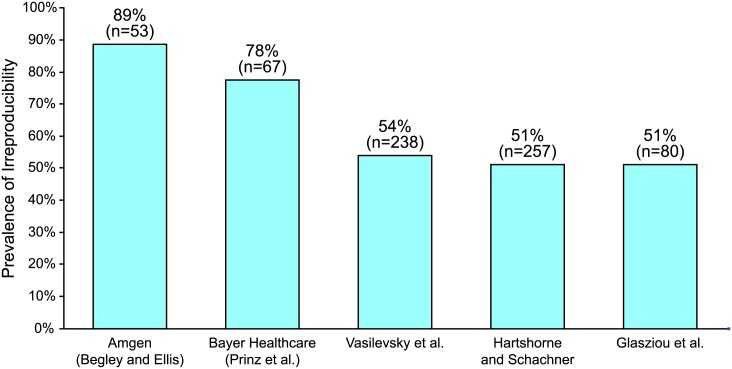
\includegraphics[width=\linewidth]{images/pbio.1002165.g001.jpg}
	\caption{Source: reproducibility crisis rates across multiple studies \cite{FreedmanLeonardetal2015}}
	\label{fig:FreedmanLeonardetal2015fig}
\end{figure}

The same article goes on to list systemic causes of irreproducibility" as being "(1) study design, (2) biological reagents and reference materials, (3) laboratory protocols, and (4) data analysis and reporting." I found it surprising that lack of access to the same or, at least, similar technology that was used in the original study was not mentioned as a probable cause, but maybe that's included in the option labeled "laboratory protocols"... 

In any case, regardless of "the cause", the bottom-line is that \textbf{it's really hard to reproduce the same results that confirm what other studies found}.

As a matter of fact, it's not only hard to reproduce, few studies even provide the right conditions so that other researchers can try to replicat their findings. "349 randomly selected research 
articles from the biomedical literature published in 2015-2018 (Serghiou et al., 2021) found that 33 (10\%) included a reproducibility component in their research" \cite{CobeyKelly2023}


\subsection{What can we do?}
While knowledge is fragile, the process of \textbf{improving one's knowledge can be antifragile}!
By systematically improving our understanding of how a system works by both \emph{via negativa} (what does not work) and \emph{via positiva} (what seems to work) - while leaving the door open for refutation to come in and prove us wrong.

This is what the next section entitled Antifragile Learning expands on.
